\chapter{Reference Models}
\label{chap:background}
\chaptermark{Reference Models}

% First draft requested by the author on 2026-11-05.
% Mathematical definitions are literature-backed or explicit descriptions of
% the pinned reference implementation. No experimental results are introduced.

\section{Anomaly detection in time series}
\label{sec:background-anomalies}
An anomaly is an observation, or a group of observations, that departs from
the behavior considered normal for the system under study. This definition
depends on the application: a statistical deviation becomes relevant when it
conflicts with the expected operation of the system. For telemetry, the
reference behavior can depend on operating modes, commands and temporal
relationships among measurements~\cite{Chandola2009AnomalySurvey,Hundman2018Spacecraft}.

We represent an observation at time index \(t\) by a row vector
\(\mathbf{x}_t\in\mathbb{R}^{F}\), where \(F\) is the number of numerical input
features. A univariate series has \(F=1\); a multivariate series has \(F>1\).
Features can include measured quantities and numerical encodings of additional
information. Their units and scales must be considered before combining them
in a reconstruction error. In the following model equations, inputs are
normalized and the corresponding errors are dimensionless.

A finite temporal context is supplied through the sliding window defined in
Equation~\eqref{eq:background-window}:
\begin{equation}
  \mathbf{W}_t =
  \begin{bmatrix}
    \mathbf{x}_{t-w+1}\\
    \vdots\\
    \mathbf{x}_{t}
  \end{bmatrix}
  \in \mathbb{R}^{w\times F}.
  \label{eq:background-window}
\end{equation}
Here, \(w\) is the window length in samples and \(\mathbf{W}_t\) contains the
observations ending at index \(t\). Its rows are samples and its columns are
features. Padding conventions for the beginning of a series, and the treatment
of separate telemetry fragments, are specified in Chapter~\ref{chap:datasets}.
No observation later than \(t\) appears in this window.

Anomalies are commonly classified as point, contextual or
collective~\cite{Chandola2009AnomalySurvey}. A point anomaly is an individual
observation that is unusual relative to the reference distribution. A
contextual anomaly is unusual only within a specified context; for example, a
sensor value can be plausible during a maneuver but unexpected during a stable
operating period. A collective anomaly is a sequence whose joint behavior is
unusual, even if its individual values are not. A persistent constant reading
can belong to this category when normal behavior requires variation. These
categories describe different aspects of an event and need not be exclusive.

Models can learn the expected behavior of a system from nominal
observations and identify anomalies by comparing their outputs
with the observed measurements~\cite{Hundman2018Spacecraft}.
A reconstruction loss does not require anomaly labels, but the
training data can still be selected as nominal.

The annotation granularity is a separate issue. A point label identifies the
status assigned to a sample, whereas a fragment label describes an interval as
a whole. The \ac{OPS-SAT} data discussed in Chapter~\ref{chap:introduction}
provide fragment annotations~\cite{Ruszczak2025OPSSAT}. Repeating such a label
on every sample makes pointwise calculations possible, but does not supply a
measured anomaly onset within that fragment.

\section{Reconstruction-based detection and anomaly scores}
\label{sec:background-reconstruction}

A reconstruction model learns to reproduce observed data.
In an autoencoder, an encoder maps the input to an internal
representation, and a decoder uses this representation to
reconstruct the input~\cite{Goodfellow2016DeepLearning}.
The reconstruction error can then be used as an anomaly
score~\cite{Tuli2022TranAD}.
It is important to state the underlying assumption: a model trained on nominal data
will reconstruct nominal observations more accurately than
anomalous ones.

In the implementation used here, the model receives the window
$\mathbf{W}_t$ and reconstructs its last sample
$\mathbf{x}_t$~\cite{TranADPlusReferenceCode}.
We describe this mapping as

\begin{equation}
  \widehat{\mathbf{x}}_t = f_{\theta}(\mathbf{W}_t).
  \label{eq:background-reconstruction}
\end{equation}

Here, $f_{\theta}$ represents the model with trainable parameters
$\theta$, while $\widehat{\mathbf{x}}_t$ is the reconstructed sample.
The target $\mathbf{x}_t$ is already included in the input window.
This means that the task is therefore to reconstruct an observed value, rather than
predict a future one.

We calculate the anomaly score as the mean squared reconstruction
error across the input features:

\begin{equation}
  s_t = \frac{1}{F}\sum_{j=1}^{F}
  \left(\widehat{x}_{t,j}-x_{t,j}\right)^2.
  \label{eq:background-mse-score}
\end{equation}

Here, $F$ is the number of features, while $x_{t,j}$ and
$\widehat{x}_{t,j}$ are the observed and reconstructed values
of feature $j$. The inputs are normalized before processing:
the reference implementation rescales each feature with the minimum
and maximum of the training data, without clipping~\cite{TranADPlusReferenceCode}.
Test observations can therefore fall outside the interval $[0,1]$,
whereas the output layer of TranAD+ (Section~\ref{sec:background-tranadplus})
is restricted to this interval.
Averaging the errors produces a single score for each sample,
following the approach described in
TranAD+~\cite{Yermakov2025TranADPlus}.

It is important to keep in mind that an
autoencoder with sufficient capacity can learn to copy its
inputs without learning useful properties of the
data~\cite{Goodfellow2016DeepLearning}.
For anomaly detection, accurate reconstruction is useful only
if the resulting scores distinguish nominal from anomalous
observations. Small reconstruction errors alone do not guarantee
this distinction.

A threshold converts the score into a binary prediction:

\begin{equation}
  \widehat{y}_t = \mathbb{1}\!\left[s_t>\tau\right].
  \label{eq:background-threshold}
\end{equation}

Here, $\tau$ is the threshold and $\mathbb{1}$ is the indicator
function. The predicted label $\widehat{y}_t$ is $1$ when the score
exceeds the threshold and $0$ otherwise.

Changing the threshold changes the predictions without changing
the trained model. Post-processing can also change the reported
metrics without changing the reconstruction errors.

\section{TranAD}
\label{sec:background-tranad}

TranAD is a transformer-based model developed for anomaly detection
in multivariate time series~\cite{Tuli2022TranAD}.
Its reconstruction process uses attention to combine information
from different positions in a sequence, with weights calculated
from the input representations~\cite{Vaswani2017Attention}.
Self-attention relates positions within the same sequence, while
cross-attention uses information from another sequence.

In an encoder--decoder architecture, the encoder builds internal
representations of the input, which the decoder uses to produce
an output. Attention is combined with feed-forward layers that
apply the same transformation separately at each sequence position;
their intermediate width is called the feed-forward dimension.
Positional information is also supplied so that the model can
account for the order of the samples~\cite{Vaswani2017Attention}.

The published TranAD architecture combines a representation of
the history up to the current time with a local input window.
A complete-sequence encoder processes the history, while a window
encoder combines local information with this broader context.
Two decoders produce reconstructions, as shown in
Figure~\ref{fig:background-tranad}~\cite{Tuli2022TranAD}.

\begin{figure}[htbp]
  \centering
  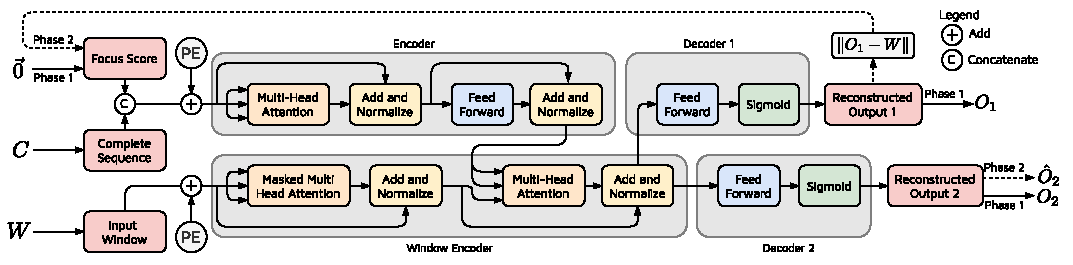
\includegraphics[width=\linewidth]{chapter2/tranad-original.pdf}
  \caption{TranAD architecture, reproduced from Figure 1
  of Tuli et al.~\cite{Tuli2022TranAD}.
  \(C\) denotes the available history, \(W\) the input window,
  and PE the positional encoding.}
  \label{fig:background-tranad}
\end{figure}
% Source: docs/papers/TranAD.pdf, Fig. 1, printed p. 1204 / PDF p. 4.

Reconstruction takes place in two phases: the first produces
an initial reconstruction, whose error becomes a focus signal
for the second. This process, called \textit{self-conditioning}, allows
the second reconstruction to depend on the errors found
in the first, without requiring anomaly labels.

The published training procedure combines reconstruction losses
with an adversarial objective, in which the two decoders have
opposing objectives for the second-phase reconstruction
error~\cite{Tuli2022TranAD}.

\section{TranAD+}
\label{sec:background-tranadplus}

\subsection{Reference architecture and training objective}
\label{sec:background-tranadplus-training}

The reference model used in this thesis is TranAD+, introduced
by Yermakov et al. and built on TranAD for anomaly detection
in high-bandwidth satellite communications~\cite{Yermakov2025TranADPlus}.
The work is motivated by DSN monitoring data, which contain
numerical and categorical variables as well as missing values.
The aim is to support operations engineers in monitoring increasing
amounts of incoming data by adapting the preprocessing and the
model to these inputs~\cite{Yermakov2025TranADPlus}.
Among other things, the original training pipeline selected only
one track for each of the SMAP, MSL and SMD datasets, while TranAD+
uses all tracks in the training
split~\cite{TranADReferenceCode,TranADPlusReferenceCode}.

The model contains a transformer encoder, two transformer decoders
and an output layer consisting of a linear transformation followed
by a sigmoid. The same encoder and output layer are used in both
processing passes, while the two decoders have separate parameters.
Figure~\ref{fig:background-tranadplus-flow} shows these components
and their connections.

\begin{figure}[htbp]
  \centering
  % Source: original TranAD+ Fig. 1 for topology; models.py:34--60 and
  % helpers.py:667--670 for exact sharing, focus and current-point query.
  \begin{tikzpicture}[
    x=1cm,y=1cm,>=Stealth,font=\small,
    block/.style={draw,rounded corners=2pt,align=center,
      minimum height=1.05cm,inner sep=5pt},
    input/.style={block,fill=black!8,minimum width=2.6cm},
    encoder/.style={block,fill=blue!10,minimum width=2.2cm},
    decoder/.style={block,fill=black!12,minimum width=2.5cm},
    head/.style={block,fill=blue!10,minimum width=2.4cm},
    output/.style={block,fill=black!8,minimum width=2.6cm},
    data/.style={->,semithick},
    sharing/.style={dashed,black!65},
    feedback/.style={->,dashed,semithick},
    note/.style={font=\footnotesize,fill=white,inner sep=2pt}
  ]
    \node[input] (in1) at (1.30,0)
      {Window $\mathbf{W}_t$\\Zero focus $\mathbf{0}$};
    \node[encoder] (en1) at (4.55,0) {Encoder\\$E$};
    \node[decoder] (de1) at (7.60,0)
      {Decoder $D_1$\\query $\mathbf{q}_t$};
    \node[head] (hd1) at (10.70,0) {Output head\\$P$};
    \node[output] (ou1) at (14.00,0)
      {Reconstruction\\$\widehat{\mathbf{x}}_t^{(1)}$};

    \node[input] (in2) at (1.30,-2.70)
      {Window $\mathbf{W}_t$\\Focus $\mathbf{C}^{(1)}_t$};
    \node[encoder] (en2) at (4.55,-2.70) {Encoder\\$E$};
    \node[decoder] (de2) at (7.60,-2.70)
      {Decoder $D_2$\\query $\mathbf{q}_t$};
    \node[head] (hd2) at (10.70,-2.70) {Output head\\$P$};
    \node[output] (ou2) at (14.00,-2.70)
      {Reconstruction\\$\widehat{\mathbf{x}}_t^{(2)}$};

    \node[anchor=west,font=\small\bfseries] at (0,0.91) {Pass 1};
    \node[anchor=west,font=\small\bfseries] at (0,-1.79) {Pass 2};
    \foreach \a/\b in {in1/en1,en1/de1,de1/hd1,hd1/ou1,
                       in2/en2,en2/de2,de2/hd2,hd2/ou2}
      \draw[data] (\a) -- (\b);
    \draw[sharing] (en1.south) --
      node[note,midway] {shared weights} (en2.north);
    \draw[sharing] (hd1.south) --
      node[note,midway] {shared weights} (hd2.north);
    \draw[feedback] (ou1.east) -- (15.90,0) -- (15.90,-4.12)
      -- node[note,midway]
      {$C^{(1)}_{t,k,j}=(\widehat{x}_{t,j}^{(1)}-W_{t,k,j})^2$}
      (1.30,-4.12) -- (in2.south);
  \end{tikzpicture}
  \caption{Computation in the TranAD+ reference implementation.
  The repeated \(E\) and \(P\) blocks are calls to the same encoder and
  output head; \(D_1\) and \(D_2\) have separate parameters. The return
  path constructs the focus for the second pass. Each decoder also
  receives the duplicated current sample \(\mathbf{q}_t\). Schematic
  derived from Figure 1 of Yermakov et al.~\cite{Yermakov2025TranADPlus}
  and the inspected implementation~\cite{TranADPlusReferenceCode}.}
  \label{fig:background-tranadplus-flow}
\end{figure}

In the first pass, the encoder receives the input window together
with a matrix of zeros, and the first decoder produces a
reconstruction of the last sample: this reconstruction is then
compared with every sample in the window, using squared differences
to construct the focus matrix. The same encoder processes the
window again with this focus, and the second decoder produces
another reconstruction. Both decoders also receive the current
sample as an input~\cite{TranADPlusReferenceCode}.

During training, the model minimizes a weighted sum of the two
reconstruction errors:

\begin{equation}
  \mathcal{L}_{n} =
  \frac{1}{n}\operatorname{MSE}
  \left(\widehat{\mathbf{x}}^{(1)}_t,\mathbf{x}_t\right)
  +
  \left(1-\frac{1}{n}\right)\operatorname{MSE}
  \left(\widehat{\mathbf{x}}^{(2)}_t,\mathbf{x}_t\right),
  \label{eq:background-tranadplus-loss}
\end{equation}

where $n\geq1$ is the training epoch, while
$\widehat{\mathbf{x}}^{(1)}_t$ and
$\widehat{\mathbf{x}}^{(2)}_t$ are the two reconstructions.
The mean squared error is averaged over features and batch
elements. Only the first reconstruction contributes directly
to the loss in the first epoch; the weight of the second
increases in subsequent epochs~\cite{TranADPlusReferenceCode}.
% Source: TranADPlus/src/helpers.py:831--849; one-based epoch n.

During evaluation, the two reconstructions are combined as

\begin{equation}
  \widehat{\mathbf{x}}_t(\alpha) =
  \alpha\widehat{\mathbf{x}}^{(1)}_t
  +(1-\alpha)\widehat{\mathbf{x}}^{(2)}_t.
  \label{eq:background-tranadplus-combination}
\end{equation}

Here, $\alpha\in[0,1]$ controls the contribution of each
reconstruction. With $\alpha=1$, only the first is used,
while $\alpha=0$ selects the second.
This evaluation parameter is separate from the epoch-dependent
weights used during training~\cite{TranADPlusReferenceCode}.

The combined reconstruction is then compared with the observed
sample to calculate the anomaly score:

\begin{equation}
  s_t(\alpha)=\frac{1}{F}\sum_{j=1}^{F}
  \left[\widehat{x}_{t,j}(\alpha)-x_{t,j}\right]^2.
  \label{eq:background-tranadplus-score}
\end{equation}

The combination therefore takes place before calculating
the squared errors, rather than averaging the errors
of the two reconstructions.
% Source: TranADPlus/src/helpers.py:665--673,726 and scripts/evaluation.py.

\subsection{Changes relative to TranAD}
\label{sec:background-tranadplus-changes}

The main changes concern the feed-forward layers, the combination
of decoder outputs and the training procedure.

\begin{itemize}

  \item TranAD+ introduces an inverse bottleneck in the feed-forward
  layers to limit information loss, particularly with inputs expanded
  by categorical encoding~\cite{Yermakov2025TranADPlus}.
  The transformation first changes the width of the representation
  and then returns it to its initial value:

  \begin{equation}
    d \longrightarrow d_{\mathrm{ff}} \longrightarrow d.
    \label{eq:background-bottleneck}
  \end{equation}

  Here, $d$ is the input and output width, while $d_{\mathrm{ff}}$
  is the intermediate width. A bottleneck makes the intermediate
  representation smaller, whereas an inverse bottleneck makes it
  larger. In the implementation used here, $d=2F$ because the window
  and focus are concatenated, so an expansion occurs when
  $d_{\mathrm{ff}}>2F$~\cite{TranADPlusReferenceCode}.

  \item TranAD+ combines the two reconstructed outputs using
  adjustable weights before calculating the anomaly score.
  The coefficient $\alpha$ controls their contributions, as described
  in Equation~\eqref{eq:background-tranadplus-combination}, allowing
  the score to use either reconstruction or a combination of
  both~\cite{Yermakov2025TranADPlus,TranADPlusReferenceCode}.

  \item Unlike the adversarial training described in the TranAD
  paper, the TranAD+ implementation minimizes a weighted sum
  of reconstruction errors with non-negative weights, as given
  in Equation~\eqref{eq:background-tranadplus-loss}.
  The second reconstruction is therefore trained to reduce its
  error, rather than to increase it through an adversarial
  objective~\cite{Tuli2022TranAD,TranADPlusReferenceCode}.

  \item The original TranAD window-conversion routine produces
  two identical initial windows because of its indexing and
  replication padding. TranAD+ corrects this duplication by
  advancing the window through the
  data~\cite{TranADReferenceCode,TranADPlusReferenceCode}.

  \item The window size, feed-forward dimension, number of layers
  and training settings can be configured in the TranAD+ pipeline.
  The documentation of the reference code also states that the training
  hyperparameters were optimized~\cite{TranADPlusReferenceCode}.
  % Source: TranADPlus/README_original.md:130.

\end{itemize}

\section{Model simplification and resource-aware inference}
\label{sec:background-efficiency}

The attention and reconstruction stages described for TranAD and
TranAD+ require memory to store the model and its intermediate
representations, as well as computation to process each telemetry
window. Starting from TranAD+ as the reference, this thesis therefore
considers detection performance together with these requirements,
since future onboard use depends on the resources available
on the spacecraft.

The number of parameters provides an initial measure of model size,
but the memory needed to store them also depends on their numerical
precision, while inference requires additional space for inputs and
intermediate results~\cite{Sze2017EfficientDNN}.
The distinction between model size and computation is visible in
TranAD+ itself: its two encoder passes use the same learned weights,
but both require operations to be performed, so sharing parameters
does not remove the cost of executing them~\cite{TranADPlusReferenceCode}.

Execution time also depends on the hardware and software used,
so measurements on the available platform do not directly establish
performance on an onboard device~\cite{Sze2017EfficientDNN}.

\section{Lightweight detectors without transformers}
\label{sec:background-lightweight}

Anomaly detection does not require a sequence model. A simpler approach
describes a piece of signal, such as a fragment or a window, with a few
statistics, for example its standard deviation, range or the size of its
changes between consecutive samples. These statistics are then compared
with those of nominal data. The \ac{OPS-SAT} benchmark follows this approach:
it provides statistical features computed for each fragment and
evaluates several detectors on them, including a nearest-neighbour
detector~\cite{Ruszczak2025OPSSAT}.

A nearest-neighbour detector stores the descriptions of nominal training
pieces and assigns each new piece a score equal to its distance from the
closest stored ones: a piece unlike any nominal example receives a high
score~\cite{Chandola2009AnomalySurvey}. Linear methods instead learn a
low-dimensional subspace that contains most of the variation of nominal
data, and use the distance from this subspace as the
score~\cite{Chandola2009AnomalySurvey}. An autoencoder built from fully
connected layers is a non-linear counterpart of this idea: it compresses
the description and reconstructs it, and the reconstruction error is the
score~\cite{Goodfellow2016DeepLearning}.

These detectors contain no attention mechanism. A fully connected network
uses only matrix products and simple element-wise functions, so its
memory and computation per decision are small and fixed. We use them as
lightweight alternatives to TranAD+ and as controls for its evaluation.
